\chapter{Perancangan}
\label{chap:perancangan}

Pada bab ini akan dijelaskan mengenai perancangan aplikasi meliputi diagram kelas rinci beserta deskripsi dan fungsinya, dan perancangan antarmuka.

\section{Diagram Kelas Rinci} 
\label{sec:kelasdiagramrinci}
Diagram kelas rinci diperoleh dari hasil pengembangan diagram kelas analisis pada subbab \ref{sec:kelasdiagram}. Diagram kelas rinci dapat dilihat pada Gambar \ref{fig:4_kelas_diagram_rinci}. 

Deskripsi kelas beserta fungsi dari diagram kelas rinci tersebut adalah sebagai berikut:

\begin{enumerate}
	\item Application\\
	Kelas ini merupakan kelas yang sudah disediakan \play dan merupakan kelas Controller pada aplikasi KIRI. Atribut yang dimiliki kelas Application adalah:
	\begin{itemize}
		\item \textbf{DynamicForm dynamicForm:} objek DynamicForm yang berperan dalam mengambil nilai pada \textit{query} parameter URL. 
		\item \textbf{Comparator<ArrayList<String>{}> comparator:} objek Comparator yang berperan dalam fungsi untuk membandingkan String dalam ArrayList.
		\item \textbf{CacheApi cache:} objek CacheApi yang berperan dalam mengambil data \textit{cache} yang telah dibuat oleh aplikasi.
		
	\end{itemize}
	\textit{Method-method} yang dimiliki kelas ini merupakan \textit{action method} dengan rincian sebagai berikut:
	\begin{itemize}
		\item \textbf{public Result index()}\\
		Berfungsi untuk validasi \textit{cache} \verb!locale! dan \verb!region! serta mengarahkan pengguna ke halaman utama KIRI.\\
		\textbf{Kembalian:}  Result yang berupa Halaman utama KIRI.
		
		\item \textbf{public Result handle()}\\
		Berfungsi untuk melakukan logikal data ketika pengguna mencari rute pada KIRI.\\
		\textbf{Kembalian:}  Halaman utama KIRI dengan hasil pencarian rute.
		
		\item \textbf{public String getFromMenjangan(String start,String finish,double mw,double wm,double pt)}\\
		Berfungsi untuk mendapatkan hasil dari \url{http://newmenjangan.cloudapp.net:8000}.\\
		\textbf{Parameter:}
				\begin{itemize}
					\item \textbf{start} Koordinat lokasi awal pengguna.
					\item \textbf{finish} Koordinat lokasi akhir pengguna.
					\item \textbf{mw} Alternatif minimum walk.
					\item \textbf{wm} Alternatif walking multiplier.
					\item \textbf{pt} Alternatif penalty transfer.
				\end{itemize}
		\textbf{Kembalian:}  Hasil dari layanan web \url{http://newmenjangan.cloudapp.net:8000} dengan \textit{query} parameter.
		
		\item \textbf{public String getFromMenjangan(String start,String finish)}\\
		Berfungsi untuk mendapatkan hasil dari \url{http://newmenjangan.cloudapp.net:8000}.\\
		\textbf{Parameter:}
				\begin{itemize}
					\item \textbf{start} Koordinat lokasi awal pengguna.
					\item \textbf{finish} Koordinat lokasi akhir pengguna.
				\end{itemize}
		\textbf{Kembalian:}  Hasil dari layanan web \url{http://newmenjangan.cloudapp.net:8000} dengan \textit{query} parameter.
		
		\item \textbf{public String getFromMenjangan(String start)}\\
		Berfungsi untuk mendapatkan hasil dari \url{http://newmenjangan.cloudapp.net:8000}.\\
		\textbf{Parameter:}
				\begin{itemize}
					\item \textbf{start} Koordinat lokasi awal pengguna.
				\end{itemize}
		\textbf{Kembalian:}  Hasil dari layanan web \url{http://newmenjangan.cloudapp.net:8000} dengan \textit{query} parameter.
		
		\item \textbf{public String file\_get\_contents(String url)}\\
		Berfungsi untuk mendapatkan hasil dari URL tertentu.\\
		\textbf{Parameter:}
				\begin{itemize}
					\item \textbf{url} URL yang ingin didapatkan.
				\end{itemize}
		\textbf{Kembalian:}  Hasil dari layanan HTTP dengan URL tertentu.
		
		\item \textbf{public String getPlacesAPI(String location,String radius,String querystring)}\\
		Berfungsi untuk mendapatkan hasil JSON dari maps.googleapis.com.\\
		\textbf{Parameter:}
				\begin{itemize}
					\item \textbf{location} Lokasi yang ingin dicari(garis lintang dan garis bujur).
					\item \textbf{radius} Radius dari lokasi yang ingin dicari.
					\item \textbf{querystring} Kata yang berkaitan dengan lokasi yang ingin dicari.
				\end{itemize}
		\textbf{Kembalian:}  Hasil dari layanan HTTP menjangan dengan query parameter.
		
		\item \textbf{public String format\_traveltime(double time)}\\
		Berfungsi untuk melakukan format waktu.\\
		\textbf{Parameter:}
				\begin{itemize}
					\item \textbf{time} Waktu yang ingin diubah formatnya sesuai format lokalisasi pengguna.
				\end{itemize}
		\textbf{Kembalian:}  Hasil waktu yang sudah diformat.
		
		\item \textbf{public String retrieve\_data(String param)}\\
		Berfungsi untuk mendapatkan data dari query URL.\\
		\textbf{Parameter:}
				\begin{itemize}
					\item \textbf{param} Query yang ingin didapatkan.
				\end{itemize}
		\textbf{Kembalian:}  Data pada \textit{query} paremeter URL.
		
		\item \textbf{public boolean check\_apikey(String apikey)}\\
		Berfungsi untuk validasi \verb!apikey! yang digunakan valid atau apikey yang digunakan ada batasan alamat IP.\\
		\textbf{Parameter:}
				\begin{itemize}
					\item \textbf{apikey} Apikey yang ingin dicek.
				\end{itemize}
		\textbf{Kembalian:}  Hasil pengecekan apikey dapat dipakai atau tidak. Jika tidak dapat dipakai, akan mengembalikan hasil pesan kesalahan.
		
		\item \textbf{public String humanize\_point(String location)}\\
		Berfungsi untuk mendapatkan nama lokasi tempat dari titik koordinat lokasi.\\
		\textbf{Parameter:}
				\begin{itemize}
					\item \textbf{location} Titik koordinat lokasi.
				\end{itemize}
		\textbf{Kembalian:}  Nama lokasi tempat.
		
		\item \textbf{public String format\_distance(double distance,String locale)}\\
		Berfungsi untuk melakukan format jarak berdasarkan lokalisasi.\\
		\textbf{Parameter:}
				\begin{itemize}
					\item \textbf{distance} Jarak yang ingin diubah formatnya.
					\item \textbf{locale} Lokalisasi bahasa.
				\end{itemize}
		\textbf{Kembalian:}  Hasil distance yang sudah diformat sesuai lokalisasi.
	\end{itemize}
	\item Constants\\
	Kelas untuk mengisi variabel dengan konstanta dan berfungsi agar tidak menuliskan konstanta berulang kali dan membantu pengembangan aplikasi KIRI. Atribut yang dimiliki kelas Constants adalah:
	\begin{itemize}
		\item \textbf{Alternative[] ALTERNATIVES:} Objek \verb!Alternative! dalam \textit{array}.
		\item \textbf{Map<String,ProtoRegion> REGIONINFOS:} HashMap yang terdiri dari kunci berupa String dan berisi objek ProtoRegion.
		\item \textbf{String CACHE\_GEOCODING:} Untuk mencari atau menyimpan pada basisdata cache dengan type geocoding.
		\item \textbf{String CACHE\_SEARCHPLACE:} Untuk mencari atau menyimpan pada tabel cache dengan tipe searchplace.
		\item \textbf{String PLACES\_URL:} URL Google API untuk mencari nama lokasi tempat.
		\item \textbf{int SEARCH\_MAXRESULT} Angka untuk menentukan batas maksimal hasil pencarian.
		\item \textbf{String GMAPS\_SERVER\_KEY:} Kunci agar dapat akses Google API.
		\item \textbf{String GMAPS\_GEOCODE\_URL:} URL Google API untuk mencari geokode lokasi tempat.
		\item \textbf{String ANGKOTWEBID\_URL\_PREFIX:} Awalan URL untuk \url{http://angkot.web.id}.
		\item \textbf{String ANGKOTWEBID\_URL\_SUFFIX:} Akhiran URL untuk \url{http://angkot.web.id}.
		\item \textbf{int SPEED\_WALK:} Kecepatan jalan kaki.
		\item \textbf{String MENJANGAN\_URL:} URL untuk mengakses \url{http://newmenjangan.cloudapp.net:8000}.
		\item \textbf{String PROTO\_ATTRIBUTIONS:} Untuk menampilkan JSON dengan \textit{key} \verb!attributions!. 
		\item \textbf{String PROTO\_ERRORCODE:} Untuk mendapatkan nilai dari \textit{query} \verb!errorcode! pada protokol.
		\item \textbf{String PROTO\_LOCALE:} Untuk mendapatkan nilai dari \textit{query} \verb!locale! pada URL.
		\item \textbf{String PROTO\_LOCALE\_INDONESIA:} Nilai dari \textit{query} \verb!locale! dengan isi \verb!`id'!.
		\item \textbf{String PROTO\_LOCALE\_ENGLISH:} Nilai dari \textit{query} \verb!locale! dengan isi \verb!`en'!.
		\item \textbf{String PROTO\_LOCATION:} Untuk menyimpan pada HashMap dengan \textit{key} location.
		\item \textbf{String PROTO\_MESSAGE:} Untuk menampilkan JSON dengan \textit{key} message.
		\item \textbf{String PROTO\_MODE\_FINDROUTE:} Untuk mendapatkan nilai dari \textit{query} parameter \verb!mode! pada protokol.
		\item \textbf{String PROTO\_MODE\_REPORTERROR:} Untuk mendapatkan nilai dari \textit{query} parameter \verb!mode! pada protokol.
		\item \textbf{String PROTO\_MODE\_SEARCH:} Untuk mendapatkan nilai dari \textit{query} parameter \verb!mode! pada protokol.
		\item \textbf{String PROTO\_MODE\_NEARBYTRANSPORTS:} Untuk mendapatkan nilai dari \textit{query}  \verb!mode! pada protokol.
		\item \textbf{String PROTO\_NEARBYTRANSPORTS:} Untuk menampilkan JSON dengan \textit{key} \verb!nearbytransports!.
		\item \textbf{String PROTO\_PLACENAME:} Untuk menampilkan JSON dengan \textit{key} \verb!placename!.
		\item \textbf{String PROTO\_PRESENTATION\_DESKTOP:} Untuk mengetahui apakah aplikasi dibuka di \textit{desktop}.
		\item \textbf{String PROTO\_PRESENTATION\_MOBILE:} Untuk mengetahui apakah aplikasi dibuka di \textit{mobile}.
		\item \textbf{String PROTO\_REGION:} Untuk mendapatkan nilai dari \textit{query} parameter \verb!region!.
		\item \textbf{String PROTO\_REGION\_BANDUNG:} Region Bandung dengan kode \verb!`bdo'!.
		\item \textbf{String PROTO\_REGION\_JAKARTA:} Region Jakarta dengan kode \verb!`jkt'!.
		\item \textbf{String PROTO\_REGION\_SURABAYA:} Region Surabaya dengan kode \verb!`sby'!.
		\item \textbf{String PROTO\_REGION\_MALANG:} Region Malang dengan kode \verb!`mlg'!.
		\item \textbf{String PROTO\_ROUTESTART:} Untuk mendapatkan nilai dari \textit{query} parameter \verb!start!.
		\item \textbf{String PROTO\_ROUTINGRESULT:} Untuk menampilkan JSON dengan \textit{key} \verb!routingresult!.
		\item \textbf{String PROTO\_ROUTINGRESULTS:} Untuk menampilkan JSON dengan \textit{key} \verb!routingresults!.
		\item \textbf{String PROTO\_SEARCH\_QUERYSTRING:} Untuk mendapatkan nilai dari \textit{query} parameter \verb!querystring!.
		\item \textbf{String PROTO\_SEARCH\_RESULT:} Untuk menampilkan JSON dengan \textit{key} \verb!searchresult!.
		\item \textbf{String PROTO\_STATUS:} Untuk menampilkan JSON dengan \textit{key} \verb!status!.
		\item \textbf{String PROTO\_STATUS\_ERROR:} Untuk menampilkan JSON dengan nilai \verb!`error'!.
		\item \textbf{String PROTO\_STATUS\_OK:} Untuk menampilkan JSON dengan nilai \verb!`ok'!.
		\item \textbf{String PROTO\_STEPS:} Untuk menampilkan JSON dengan \textit{key} \verb!steps!.
		\item \textbf{String PROTO\_TRAVELTIME:} Untuk menampilkan JSON dengan \textit{key} \verb!traveltime!.
		\item \textbf{String PROTOKD\_POINT\_FINISH:} Untuk pengecekan \textit{array} \verb!point! yang didapat dari URL \url{http://newmenjangan.cloudapp.net:8000} terdapat kata kunci \verb!`finish'!.
		\item \textbf{String PROTOKD\_POINT\_START:} Untuk pengecekan \textit{array} \verb!point! yang didapat dari URL \url{http://newmenjangan.cloudapp.net:8000} terdapat kata kunci \verb!`start'!.
		\item \textbf{String PROTOKD\_RESULT\_NONE:} Untuk pengecekan \textit{array} \verb!point! yang didapat dari URL \url{http://newmenjangan.cloudapp.net:8000} terdapat kata kunci \verb!`none'!.
		\item \textbf{String PROTOKD\_TRANSITMODE\_WALK:} Untuk pengecekan \textit{array} \verb!point! yang didapat dari URL \url{http://newmenjangan.cloudapp.net:8000} terdapat kata kunci \verb!`walk'!.
	\end{itemize}
	
	
	\item Alternative\\
	Kelas yang berada pada \textit{package} models. Kelas ini untuk merepresentasikan alternatif dalam pencarian rute pada URL \textit{http://newmenjangan.cloudapp.net:8000}. Kelas Alternative mempunyai atribut antara lain:
	\begin{itemize}
		\item \textbf{double mw:} Maximumwalk dari alternatif.
		\item \textbf{double wm:} Walkingmultiplier dari alternatif.
		\item \textbf{double pt:}  Penaltrytransfer dari alternatif.
	\end{itemize}
	
	\textit{Method-method} yang dimiliki kelas ini merupakan \textit{action method} dengan rincian sebagai berikut:
	\begin{itemize}
		\item \textbf{public double getPt()}\\
		Berfungsi untuk mendapatkan atribut pt.\\
		\textbf{Kembalian:}  Nilai pt.
		
		\item \textbf{public double getWm()}\\
		Berfungsi untuk mendapatkan atribut wm.\\
		\textbf{Kembalian:}  Nilai wm.
		
		\item \textbf{public double getMw()}\\
		Berfungsi untuk mendapatkan atribut mw.\\
		\textbf{Kembalian:}  Nilai mw.
	\end{itemize}
	
	\item ProtoRegion\\
	Kelas yang berada pada \textit{package} models. Kelas ini untuk merepresentasikan kota dengan atribut masing-masing. Kelas ProtoRegion mempunyai atribut antara lain:
	\begin{itemize}
		\item \textbf{double lat:} Titik lintang dari kota tertentu.
		\item \textbf{double lon:} Titik bujur dari kota tertentu.
		\item \textbf{int radius:}  Radius dari kota tertentu.
		\item \textbf{int zoom:}  Tingkat \textit{zoom} dari kota tertentu.
		\item \textbf{String searchPlace\_regex:}  \textit{Regex} dari kota tertentu guna dalam pencarian nama lokasi.
		\item \textbf{String name:}  Nama dari kota tertentu.
	\end{itemize}
	
	\textit{Method-method} yang dimiliki kelas ini merupakan \textit{action method} dengan rincian sebagai berikut:
	\begin{itemize}
		\item \textbf{public double getLat()}\\
		Berfungsi untuk mendapatkan atribut titik lintang.\\
		\textbf{Kembalian:}  Nilai titik lintang.
		
		\item \textbf{public double getLon()}\\
		Berfungsi untuk mendapatkan atribut titik bujur.\\
		\textbf{Kembalian:}  Nilai titik bujur.
		
		\item \textbf{public int getZoom()}\\
		Berfungsi untuk mendapatkan atribut tingkat \textit{zoom}.\\
		\textbf{Kembalian:}  Nilai \textit{zoom}.
		
		\item \textbf{public int getRadius()}\\
		Berfungsi untuk mendapatkan atribut radius.\\
		\textbf{Kembalian:}  Nilai radius.
		
		\item \textbf{public String getSearchPlace\_regex()}\\
		Berfungsi untuk mendapatkan atribut \textit{regex}.\\
		\textbf{Kembalian:}  Nilai \textit{regex}.
		
		\item \textbf{public String getName()}\\
		Berfungsi untuk mendapatkan atribut nama.\\
		\textbf{Kembalian:}  Nilai nama.
	\end{itemize}
	
	\item Utils\\
	Kelas yang merupakan kelas pembantu untuk fungsi-fungsi dalam aplikasi KIRI. Kelas Utils mempunyai \textit{method-method} dengan rincian sebagai berikut:
	\begin{itemize}
	
		\item \textbf{public static void log\_statistic(String verifier,String type,String additional\_info)}\\
		Berfungsi untuk memasukkan data dalam tabel statistic.\\
		\textbf{Parameter:}
				\begin{itemize}
					\item \textbf{verifier} Apikey yang mengisi data ke tabel.
					\item \textbf{type} Tipe statistik.
					\item \textbf{additional\_info} Keterangan statistik.
				\end{itemize}.
		\textbf{Kembalian:}  Tidak ada.
	
%		\item \textbf{public static boolean pregMatch(String regex, String content)}\\
%		Berfungsi untuk pengecekan apakah dalam suatu kalimat mengandung kata tertentu.\\
%		\textbf{Parameter:}
%				\begin{itemize}
%					\item \textbf{regex} Kata yang ingin dicari.
%					\item \textbf{content} Kalimat yang ingin dicari.
%				\end{itemize}.
%		\textbf{Kembalian:}  \texttt{true} jika terdapat kata dalam kalimat, \texttt{false} jika tidak ada.
		
		\item \textbf{public static int indexPregMatch(String regex, String content)}\\
		Berfungsi untuk mengambil indeks kata tertentu dalam suatu kalimat jika ada.\\
		\textbf{Parameter:}
				\begin{itemize}
					\item \textbf{regex} Kata yang ingin dicari.
					\item \textbf{content} Kalimat yang ingin dicari.
				\end{itemize}.
		\textbf{Kembalian:}  Index kata tersebut dalam kalimat. Jika tidak ada akan mengembalikan -1.
		
		\item \textbf{public static ObjectNode die\_nice(String message)}\\
		Berfungsi untuk mengembalikan JSON dengan status error dan message.\\
		\textbf{Parameter:}
				\begin{itemize}
					\item \textbf{message} Message yang ingin dituliskan.
				\end{itemize}.
		\textbf{Kembalian:}  JSON dengan status error dan message.
		
		\item \textbf{public static ObjectNode well\_done(String message)}\\
		Berfungsi untuk mengembalikan JSON dengan status ok dan message(jika ada).\\
		\textbf{Parameter:}
				\begin{itemize}
					\item \textbf{message} Message yang ingin dituliskan.
				\end{itemize}.
		\textbf{Kembalian:}  JSON dengan status ok dan message.
		
		\item \textbf{public static String get\_from\_cache(String type, String key)}\\
		Berfungsi untuk mendapatkan nilai cacheValue dari tabel cache dengan tipe dan key tertentu.\\
		\textbf{Parameter:}
				\begin{itemize}
					\item \textbf{type} Tipe cache.
					\item \textbf{key} Key dari cache.
				\end{itemize}.
		\textbf{Kembalian:}  Nilai dari cacheValue.
	
		\item \textbf{public static void put\_to\_cache(String type, String key)}\\
		Berfungsi untuk menyimpan nilai cacheValue ke tabel cache dengan tipe dan key tertentu.\\
		\textbf{Parameter:}
				\begin{itemize}
					\item \textbf{type} Tipe cache.
					\item \textbf{key} Key dari cache.
				\end{itemize}.
		\textbf{Kembalian:}  Tidak ada.
	
%		\item \textbf{public static double deg2rad(double deg)}\\
%		Berfungsi untuk mengubah angka dalam satuan derajat dengan satuan radian.\\
%		\textbf{Parameter:}
%				\begin{itemize}
%					\item \textbf{deg} Angka dalam satuan derajat yang ingin diubah.
%				\end{itemize}.
%		\textbf{Kembalian:}  Angka dalam satuan radian.
	
		\item \textbf{public static void log\_error(String message)}\\
		Berfungsi untuk melakukan \textit{log} dengan pesan tertentu.\\
		\textbf{Parameter:}
				\begin{itemize}
					\item \textbf{message} Pesan yang ingin dikeluarkan.
				\end{itemize}.
		\textbf{Kembalian:}  Tidak ada.
		
		\item \textbf{public static String validateLocale(String locale)}\\
		Berfungsi untuk melakukan validasi locale yang didapat dari cache.\\
		\textbf{Parameter:}
				\begin{itemize}
					\item \textbf{locale} Masukan locale.
				\end{itemize}.
		\textbf{Kembalian:}  Locale yang sudah divalidasi.
		
		\item \textbf{public static String validateRegion(String region)}\\
		Berfungsi untuk melakukan validasi region yang didapat dari cache.\\
		\textbf{Parameter:}
				\begin{itemize}
					\item \textbf{region} Masukan region.
				\end{itemize}.
		\textbf{Kembalian:}  Region yang sudah divalidasi.
		
	\end{itemize}
	
	\item Index.scala.html\\
	Kelas yang berada pada package views dan berfungsi untuk tampilan pada aplikasi KIRI.
	
\end{enumerate}


\begin{figure}[H]
	\centering
	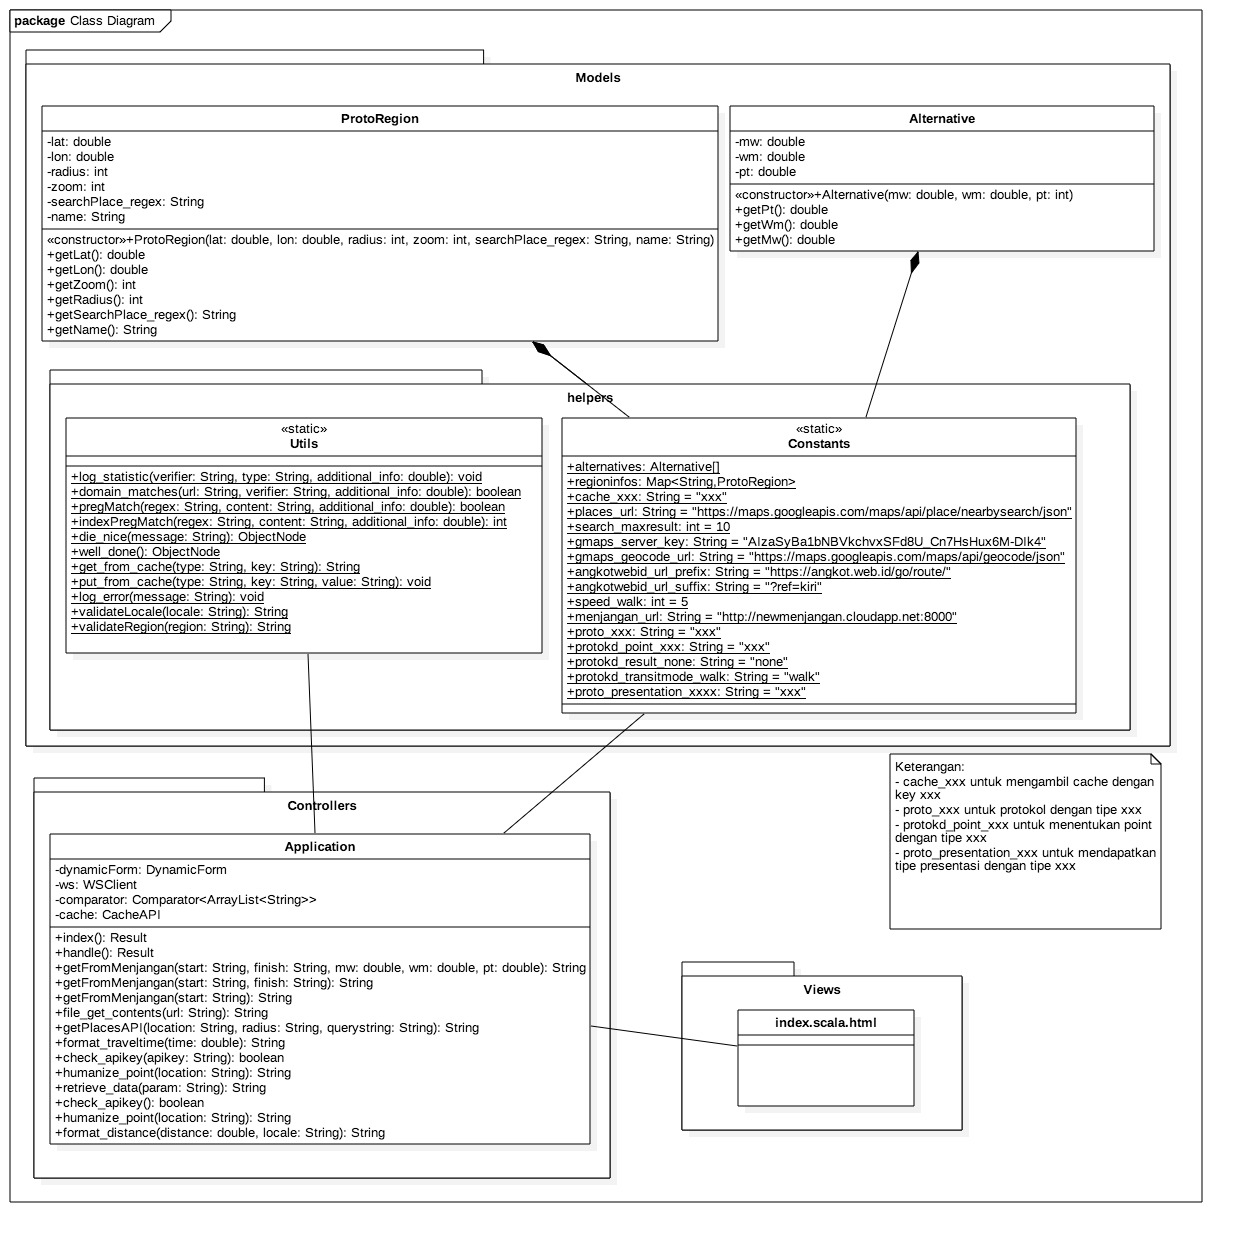
\includegraphics[scale=0.4]{Gambar/Class-Diagram-Rinci}
	\caption{Diagram Kelas Rinci} 
	\label{fig:4_kelas_diagram_rinci}
\end{figure}


\section{Perancangan Antarmuka}
\label{sec:perancangan_antarmuka}

Untuk memenuhi kebutuhan interaksi antara pengguna dengan sistem, maka sebuah antarmuka mengikuti aplikasi KIRI yang lama. Antarmuka terdiri dari:

\begin{figure}[H]
	\centering
	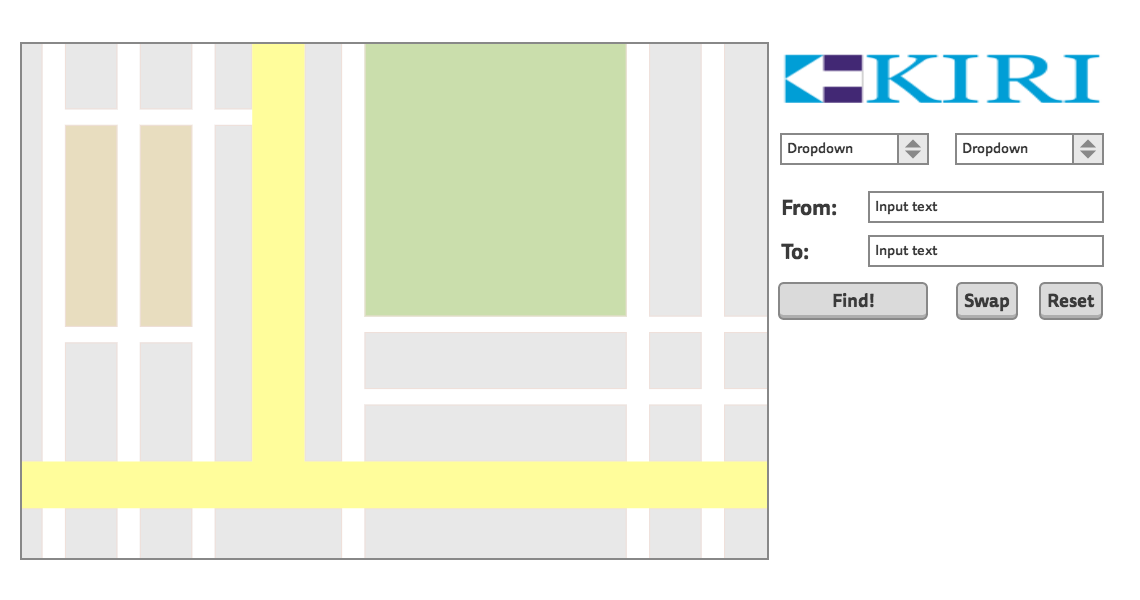
\includegraphics[scale=0.3]{Gambar/mockup-home}
	\caption{Halaman Utama KIRI} 
	\label{fig:4_KIRI_main}
\end{figure}

Pada halaman utama KIRI (dapat dilihat pada gambar \ref{fig:4_KIRI_main}), terdapat beberapa bagian yaitu:
    \begin{enumerate}
    		\item \textbf{Peta}
    		\item \textbf{Form Samping} yang terdiri dari beberapa bagian, yaitu:
    		\begin{enumerate}
    			\item Dropdown Menu Kota
    			\item Dropdown Menu Bahasa
    			\item Textfield
    			\item Tombol Swap
    			\item Tombol Reset
    			\item Tombol Find
    		\end{enumerate}
    \end{enumerate}

\subsection{Peta}
Peta berfungsi untuk memudahkan pengguna dalam memilih lokasi awal dan lokasi akhir serta memberikan gambaran rute yang telah dicari oleh KIRI. KIRI menggunakan OpenLayers yang berbasis JavaScript untuk memuat peta pada halaman web. 

\subsection{Form Samping}
\textit{Form} yang terdapat pada halaman utama KIRI (Gambar \ref{fig:4_KIRI_form}) terdiri dari:
\begin{figure}[H]
	\centering
	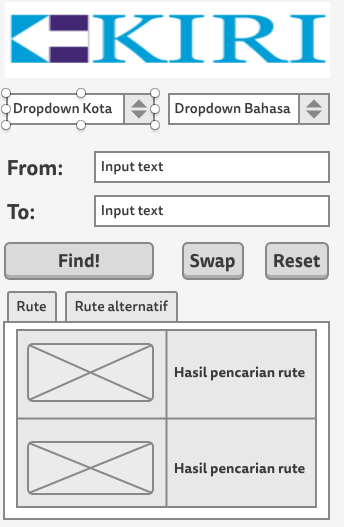
\includegraphics[scale=0.5]{Gambar/mockup-form}
	\caption{Form pada KIRI} 
	\label{fig:4_KIRI_form}
\end{figure}

\subsubsection{Dropdown Menu Kota}
\textit{Dropdown} yang berfungsi untuk memilih kota yang akan ditampilkan pada peta dan memperbarui peta.

\subsubsection{Dropdown Menu Bahasa}
\textit{Dropdown} yang berfungsi untuk memilih bahasa yang akan digunakan pada aplikasi KIRI.


\subsubsection{Textfield}
\textit{Textfield} pada KIRI agar pengguna dapat memasukkan \textit{input} sendiri. Textfield pada KIRI dapat menerima dua masukan pengguna, yaitu:

\begin{enumerate}
	\item \textbf{Textfield dengan Masukan Nama Tempat}, pengguna dapat memasukkan nama tempat asal dan tujuan.
	
	\item \textbf{Textfield dengan Masukan Klik Peta}, pengguna memasukkan koordinat tempat asal dan tujuan dengan klik pada peta. Dengan melakukan klik pada peta, textfield tempat asal dan tujuan akan akan secara otomatis terisi oleh koordinat masing-masing tempat.
	

\end{enumerate}

\subsubsection{Tombol Swap}
Pengguna dapat menukar isi dari \textit{textfield} tempat asal dan tujuan. 

\subsubsection{Tombol Reset}
Pengguna dapat melakukan pemilihan tempat dari awal dan mengulang tampilan peta. 

\subsubsection{Tombol Find}
Pengguna dapat mencari rute untuk sampai ke tujuan (Gambar \ref{fig:4_KIRI_find}). Pengguna dapat memilih rute alternatif yang sudah disediakan KIRI jika ada.

\begin{figure}[H]
	\centering
	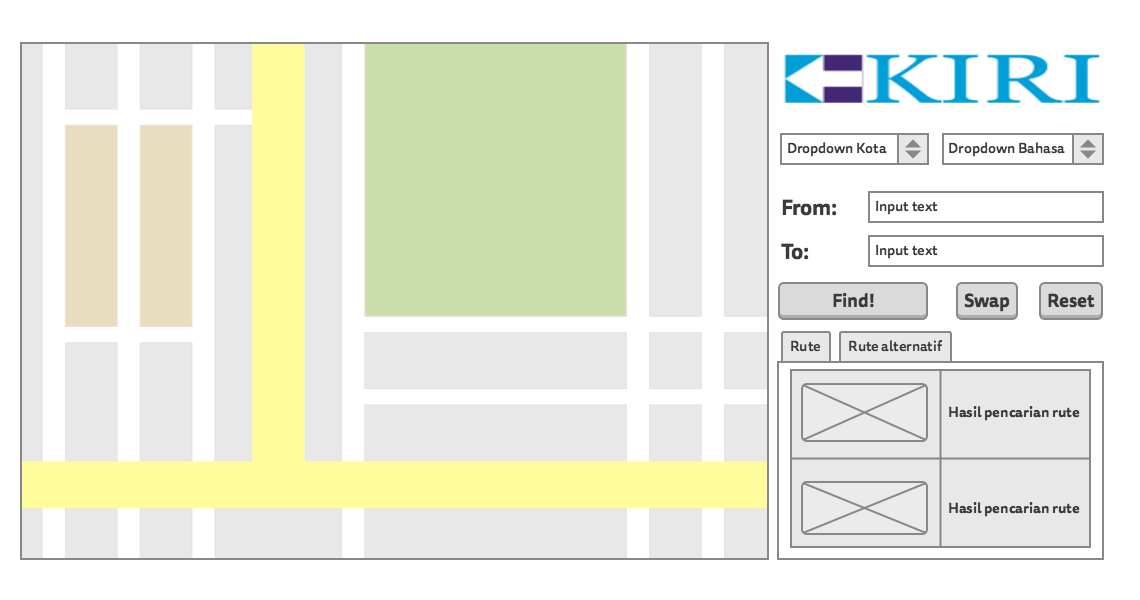
\includegraphics[scale=0.3]{Gambar/mockup-findroute}
	\caption{Contoh Pencarian Rute pada KIRI} 
	\label{fig:4_KIRI_find}
\end{figure}
